\section{Introduction}

With the development of computing technology, data storage usage continues to grow to high values. The development of data usage and storage is driven by the emergence of cloud computing technology, data needs for artificial intelligence training based on machine learning, and general improvement in data quality in files.

Along with this, the use of systems has become increasingly intensive. This intensive use creates a need for high resilience so that these systems can continue to operate, especially in facing the possibility of component failure and data loss \cite{weatherspoon2002erasure}. In this case, data redundancy solutions become very important. Traditionally, replication techniques are used to duplicate data to multiple nodes. However, with the growing need for data in operations, this approach consumes increasingly large storage capacity and significantly increases operational costs.

Another solution to address these failures is erasure coding. With the application of erasure coding, data storage requirements can be reduced while maintaining data integrity and resilience, especially in distributed system environments using multiple devices simultaneously \cite{balaji2018erasure}. However, erasure coding requires higher computational resources compared to replication in its implementation. This causes high latency and response time from the services created. In fact, many application services make low latency a requirement in their operations \cite{dean2013tail}.

The fundamental trade-off can be expressed mathematically. For write operations, the total response time for erasure coding ($T_{EC}$) versus replication ($T_{REP}$) can be modeled as:

\begin{equation}
T_{EC} = T_{encoding} + T_{network\_reduced} + T_{consensus}
\end{equation}

\begin{equation}
T_{REP} = T_{network\_full} + T_{consensus}
\end{equation}

Where $T_{network\_reduced} < T_{network\_full}$ due to the smaller total data volume transmitted in erasure coding, but $T_{encoding} > 0$ represents the computational overhead. The performance crossover occurs when $T_{EC} < T_{REP}$.

However, besides adding computation, the application of erasure coding in a system reduces the overall data size to provide data integrity and resilience. For resilience of $t$ and node count of $k$, reed-solomon based erasure coding systems has a storage ratio compared to replication that can be expressed as:

\begin{equation}
	R = \frac{\text{Message Size} \times (t + 1)}{\text{Message Size} \times \frac{\text{k + t}}{k}}
	\label{eq:erasure_storage}
\end{equation}

\begin{equation}
	R = \frac{k + kt}{k + t}
\end{equation}

Reducing data size can also cause a decrease in the size of data sent to other nodes. Thus, erasure coding has the potential to have conditions when the data size is large enough and the network is slow enough that the response time is lower in certain operations compared to performing the same operations on a replication system.

\section{Related Work}

Several studies have explored the application of erasure coding in distributed storage systems. Weatherspoon and Kubiatowicz \cite{weatherspoon2002erasure} demonstrated the effectiveness of erasure codes in providing fault tolerance with lower storage overhead compared to replication. Balaji et al. \cite{balaji2018erasure} analyzed the trade-offs between storage efficiency and computational overhead in erasure-coded systems.

Other researches have shown that erasure coding indeed has an impact on distributed systems compared to replication \cite{mu2014paxos} \cite{wang2020craft}. But these researches did not sufficiently show where the two approaches diverge in terms of performance metrics and did not provide an open-source implementation for further exploration.

\section{System Design and Implementation}

\subsection{Architecture Overview}

The implemented distributed key-value store system employs a modular architecture designed to support both erasure coding and replication mechanisms under identical conditions. The system consists of several key components:

\begin{itemize}
\item \textbf{Node}: Basic computational unit managing data storage, retrieval, and consensus operations
\item \textbf{Data Collector}: External benchmarking system for systematic performance data collection
\item \textbf{Benchmark Component}: Automated testing framework with configurable parameter variations
\item \textbf{In-memory Key-Value Store}: High-performance cache layer to optimize read operations
\item \textbf{Persistent Database}: RocksDB-based storage layer for durability
\item \textbf{Consensus Layer}: OmniPaxos protocol ensuring data consistency across distributed nodes
\end{itemize}

The system is designed to be able to test configuration differences without major changes, allowing for various experimentation regarding the comparison between erasure coding and replication.

\subsection{Erasure Coding Implementation}

The erasure coding implementation utilizes Reed-Solomon algorithms with configurable data and parity shard ratios. The encoding process transforms original data into multiple fragments, where any subset of fragments can reconstruct the original data. This approach provides fault tolerance equivalent to replication while requiring significantly less storage space.

\subsection{Consensus and Consistency}

The OmniPaxos consensus protocol used in this experimentation is modified to be able to utilize both erasure coding and replication by forking the OmniPaxos implementation repository with minimum changes on the protocol. This modified protocol enables fair performance comparison between erasure coding and replication by maintaining identical consistency guarantees. The modified protocol should have the same performance characteristics as the original OmniPaxos implementation by Ng \cite{ng2023omni}.

\subsection{Performance Monitoring and Tracing}

Additionally, the system incorporates partial performance monitoring capabilities:
\begin{itemize}
\item Operation-level tracing
\item CPU usage tracking during system runtime
\end{itemize}

These monitoring capabilities allows the analysis of performance bottlenecks and validation of theoretical predictions.

\section{Experimental Setup}

\subsection{Test Environment}

The experiments are conducted on a single virtual machine with local network. The setup allows for variation in system performance with simulated network conditions. However, it is important to note that this environment may not fully capture the complexities of real-world distributed systems.

\subsection{Parameters}

There are many variables that affects the response time performance for both replicated and erasure coding based systems. This experiment varies two critical parameters:
\begin{itemize}
\item \textbf{Network Bandwidth}: 1Mbps, 10-70Mbps (incremental with 15Mbps steps), and 10Gbps
\item \textbf{Payload Size}: 1KB, 200KB-1000KB (incremental with 200KB steps)
\end{itemize}

This parameter matrix generates 25 experimental conditions which will be used for the performance analysis.

\subsection{Testing Scenarios}

The benchmark system implements three distinct testing scenarios designed to explore different operational environments:

\begin{itemize}
\item \textbf{Scenario 1 - High Performance Environment}: Simulates modern data center conditions with high bandwidth (10 Gbps) and small payloads (1KB), an extreme condition designed to favor replication performance.
\item \textbf{Scenario 2 - Resource Constrained Environment}: Models edge computing or IoT scenarios with limited bandwidth (1 Mbps) and large payloads (200-1000KB), an extreme condition designed to favor erasure coding performance.
\item \textbf{Scenario 3 - Realistic Network Conditions}: Represents typical internet connectivity with moderate bandwidth (10-70 Mbps) and variable payload sizes, designed to identify performance crossover points.
\end{itemize}

\section{Results and Analysis}

This section presents the evaluation conducted using the implemented system with three distinct scenarios designed to explore different operational environments. The analysis focuses on write and read operations performance under varying network bandwidth and payload size conditions.

\subsection{Write Operation Analysis}

The write operation analysis validates the hypothesis that erasure coding can outperform replication under specific conditions. Three scenarios were evaluated:

\textbf{Scenario 1 - High Performance Environment (10 Gbps, 1KB payload):} Results confirm replication superiority in high-bandwidth, small-payload conditions. With minimal data transfer time, computational overhead becomes the dominant factor. Erasure coding's encoding complexity results in higher response times compared to replication's simpler operations. This environment is typical of modern data center inter-server communications, as shown in Figure \ref{fig:write-smload-fastnet}.

\begin{figure}[ht]
\centering
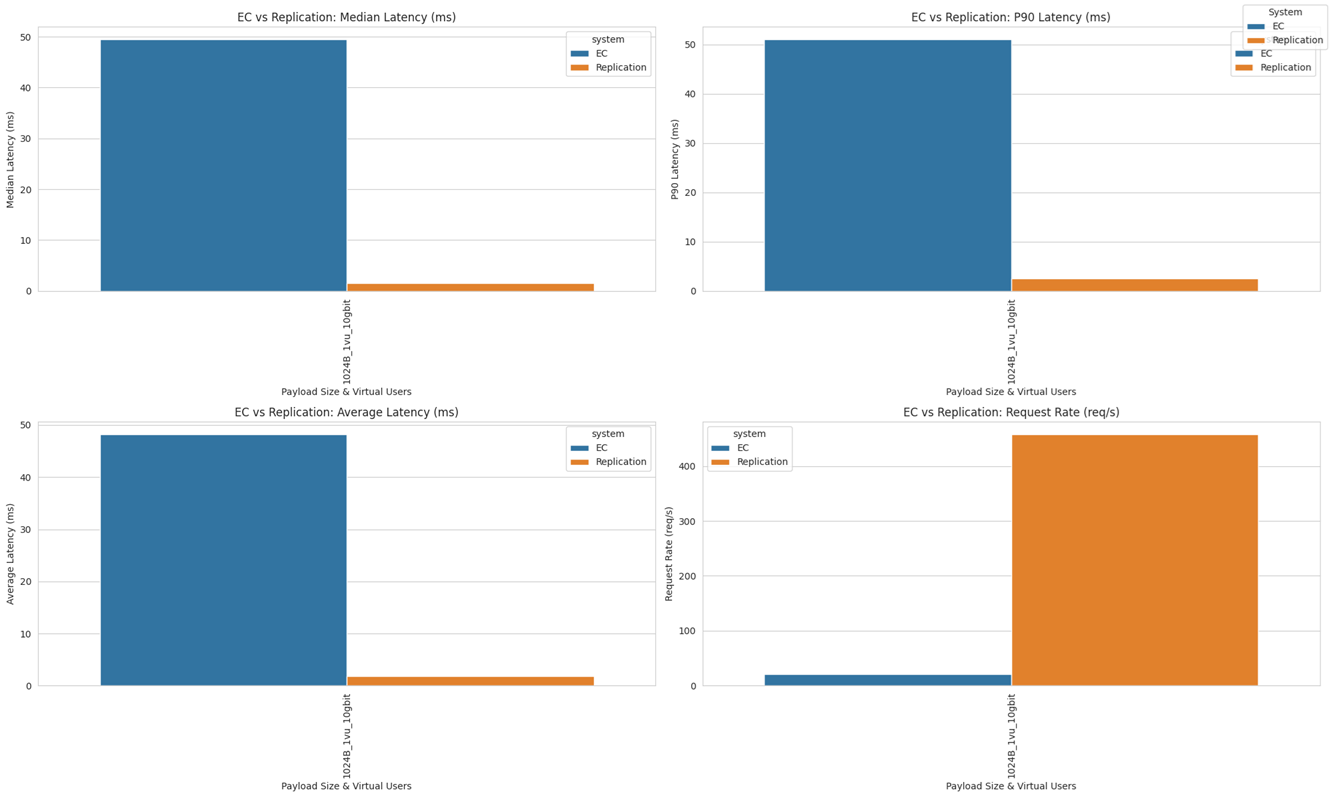
\includegraphics[width=\columnwidth]{resources/chapter-4/write_smload_fastnet.png}
\caption{Write Performance in High Bandwidth, Small Payload Environment}
\label{fig:write-smload-fastnet}
\end{figure}

\textbf{Scenario 2 - Resource Constrained Environment (1 Mbps, 200KB-1MB payload):} Results demonstrate erasure coding's advantage in bandwidth-limited scenarios with large payloads. Data transfer time becomes the dominant factor, and erasure coding's reduced data volume transmission outweighs its computational overhead. This environment represents edge computing, IoT deployments, or backup operations over limited connections, as illustrated in Figure \ref{fig:write-bigload-slownet}.

\begin{figure}[ht]
\centering
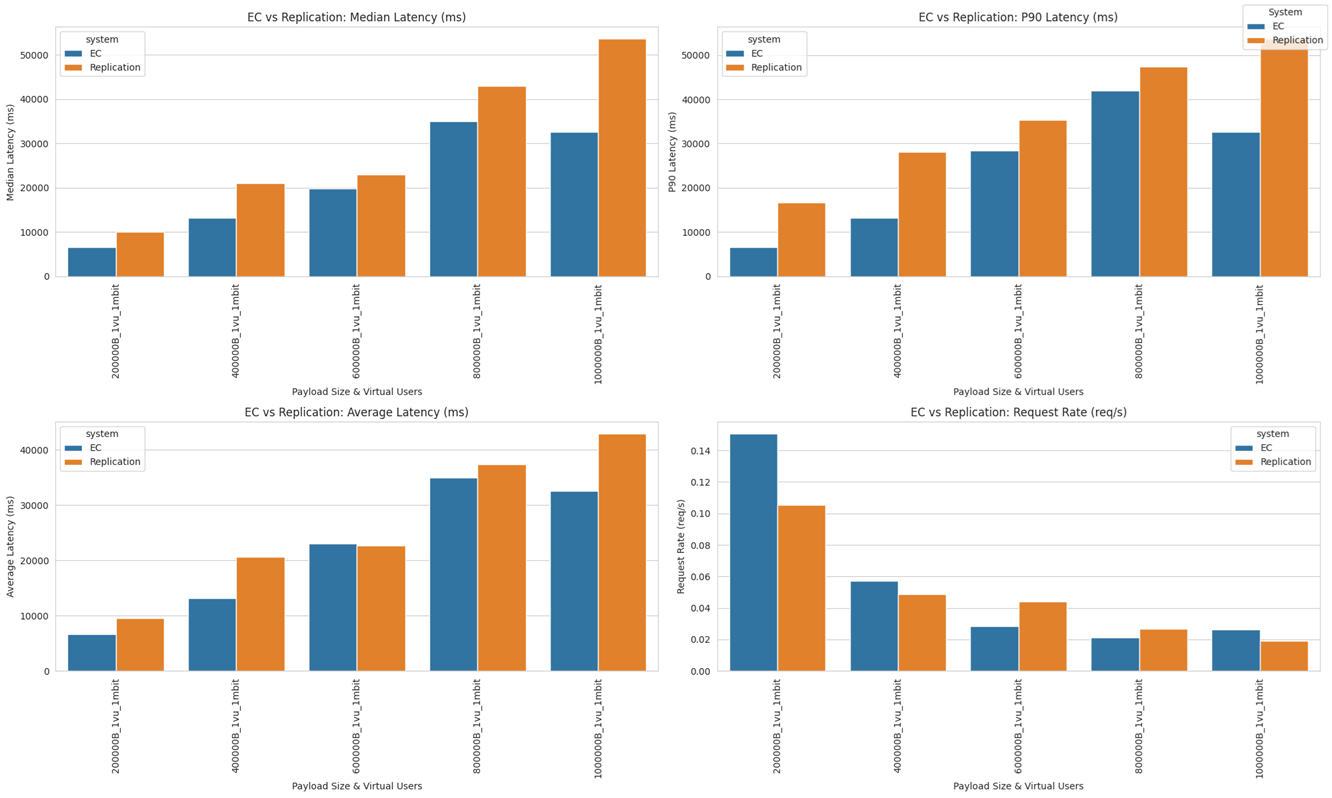
\includegraphics[width=\columnwidth]{resources/chapter-4/write_bigload_slownet.png}
\caption{Write Performance in Low Bandwidth, Large Payload Environment}
\label{fig:write-bigload-slownet}
\end{figure}

\textbf{Scenario 3 - Realistic Network Conditions (10-70 Mbps, variable payload):} This scenario reveals the performance crossover point between erasure coding and replication. Using ridge regression analysis on the 25 experimental data points, a mathematical boundary curve was derived to predict optimal system selection based on bandwidth and payload size parameters. Figure \ref{fig:write-bigload-avgnet} demonstrates the complex performance relationships in this scenario.

\begin{figure}[ht]
\centering
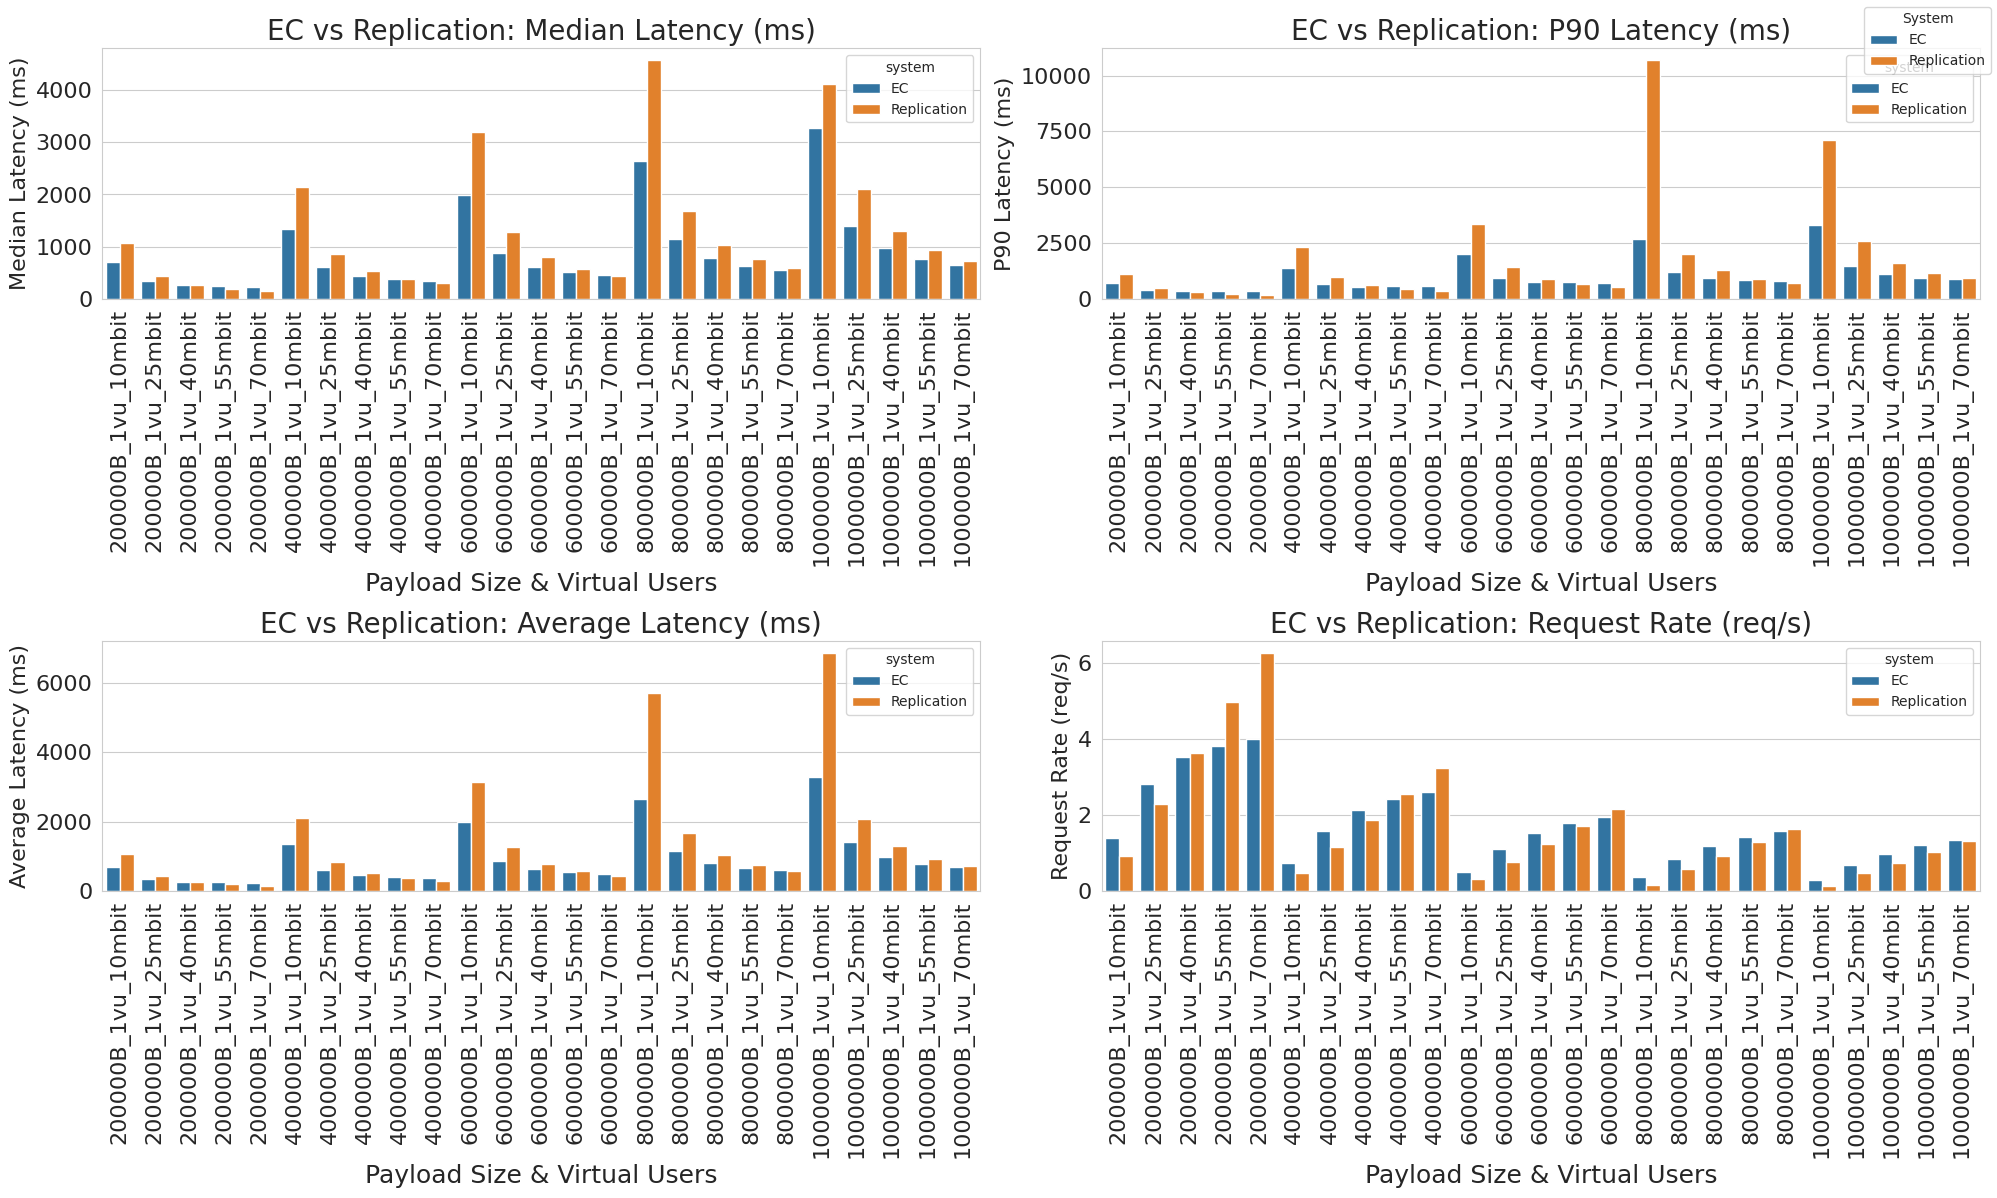
\includegraphics[width=\columnwidth]{resources/chapter-4/write_bigload_avgnet.png}
\caption{Write Performance in Moderate Bandwidth, Variable Payload Environment}
\label{fig:write-bigload-avgnet}
\end{figure}

The regression analysis produces a three-dimensional model where the intersection of erasure coding and replication performance surfaces defines the threshold boundary. Values above this curve favor erasure coding, while values below favor replication. The model accounts for the fundamental trade-off between computational overhead and network transfer efficiency.

\begin{figure}[ht]
\centering
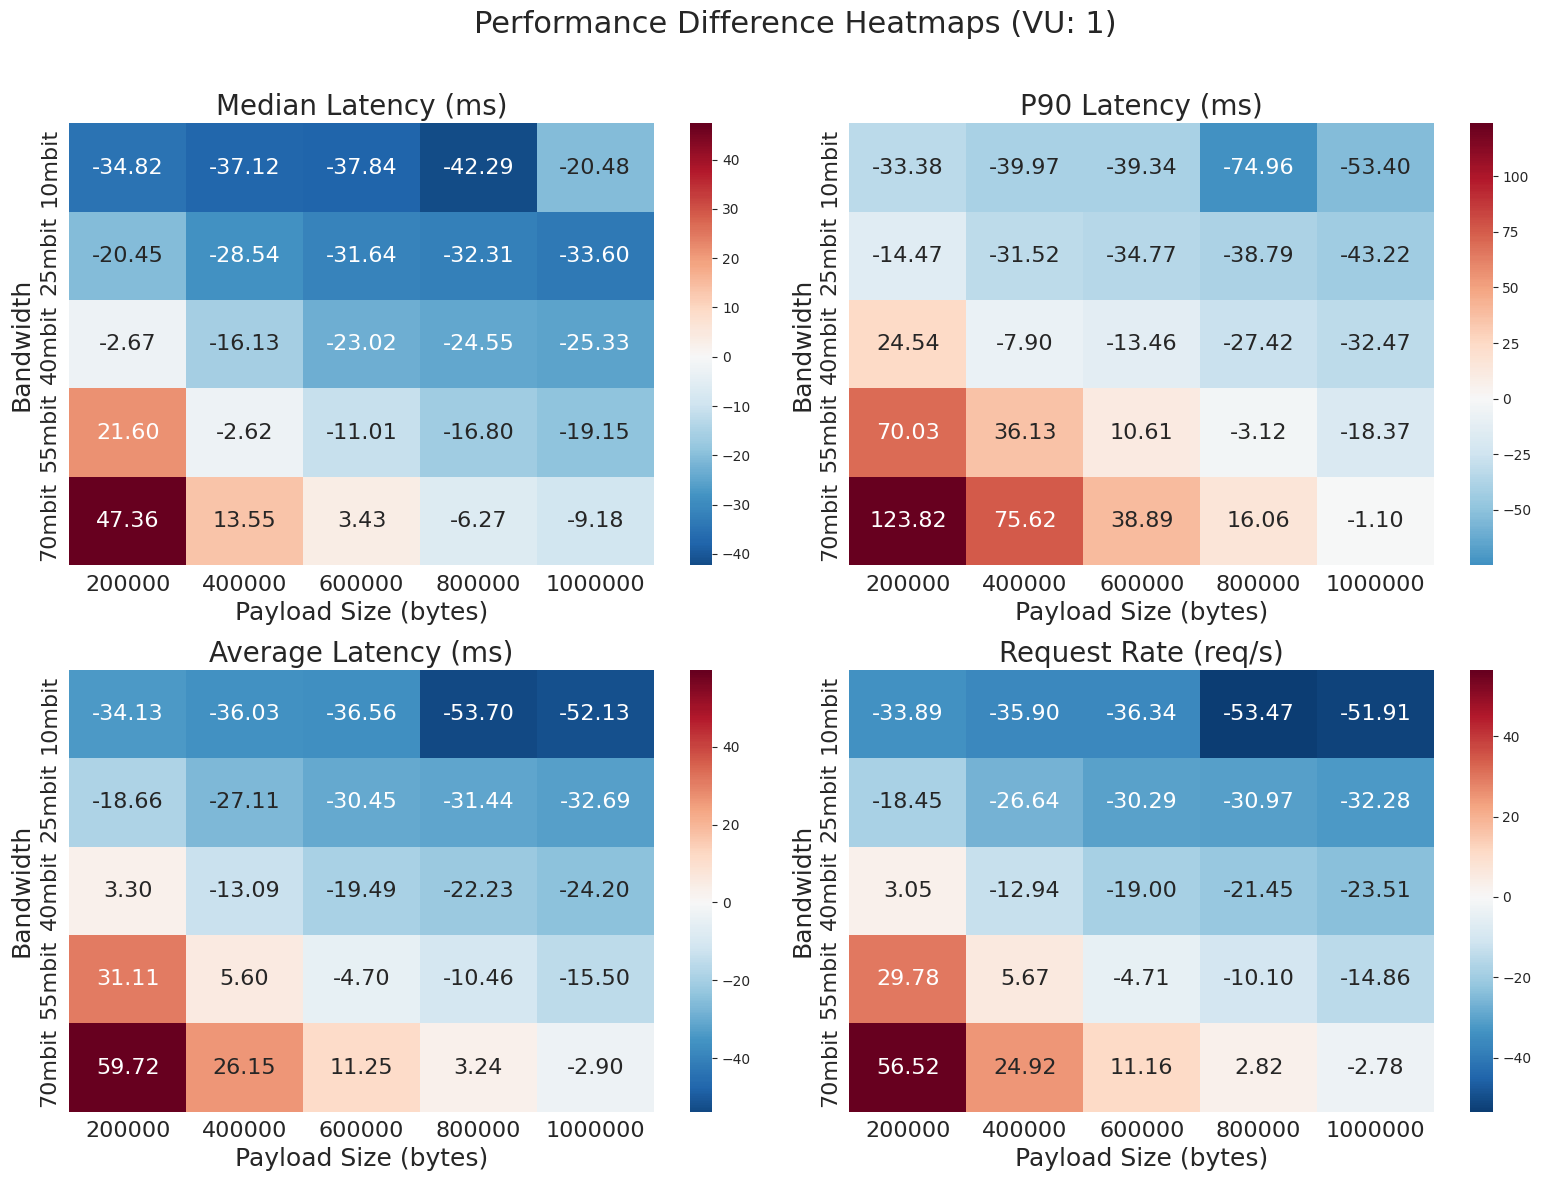
\includegraphics[width=\columnwidth]{resources/chapter-4/write_bigload_avgnet_heatmap.png}
\caption{Performance Ratio Heatmap for Write Operations}
\label{fig:write-heatmap}
\end{figure}

The heatmap visualization in Figure \ref{fig:write-heatmap} shows the performance ratio between erasure coding and replication across different bandwidth and payload combinations. Blue regions indicate conditions where erasure coding outperforms replication, while red regions favor replication. The color intensity corresponds to the magnitude of performance difference. The transition zone reveals the performance crossover boundary where system selection becomes critical. Erasure coding advantages are concentrated in low bandwidth and large payload conditions, while replication dominance occurs with high bandwidth and smaller payloads.

\begin{figure}[ht]
\centering
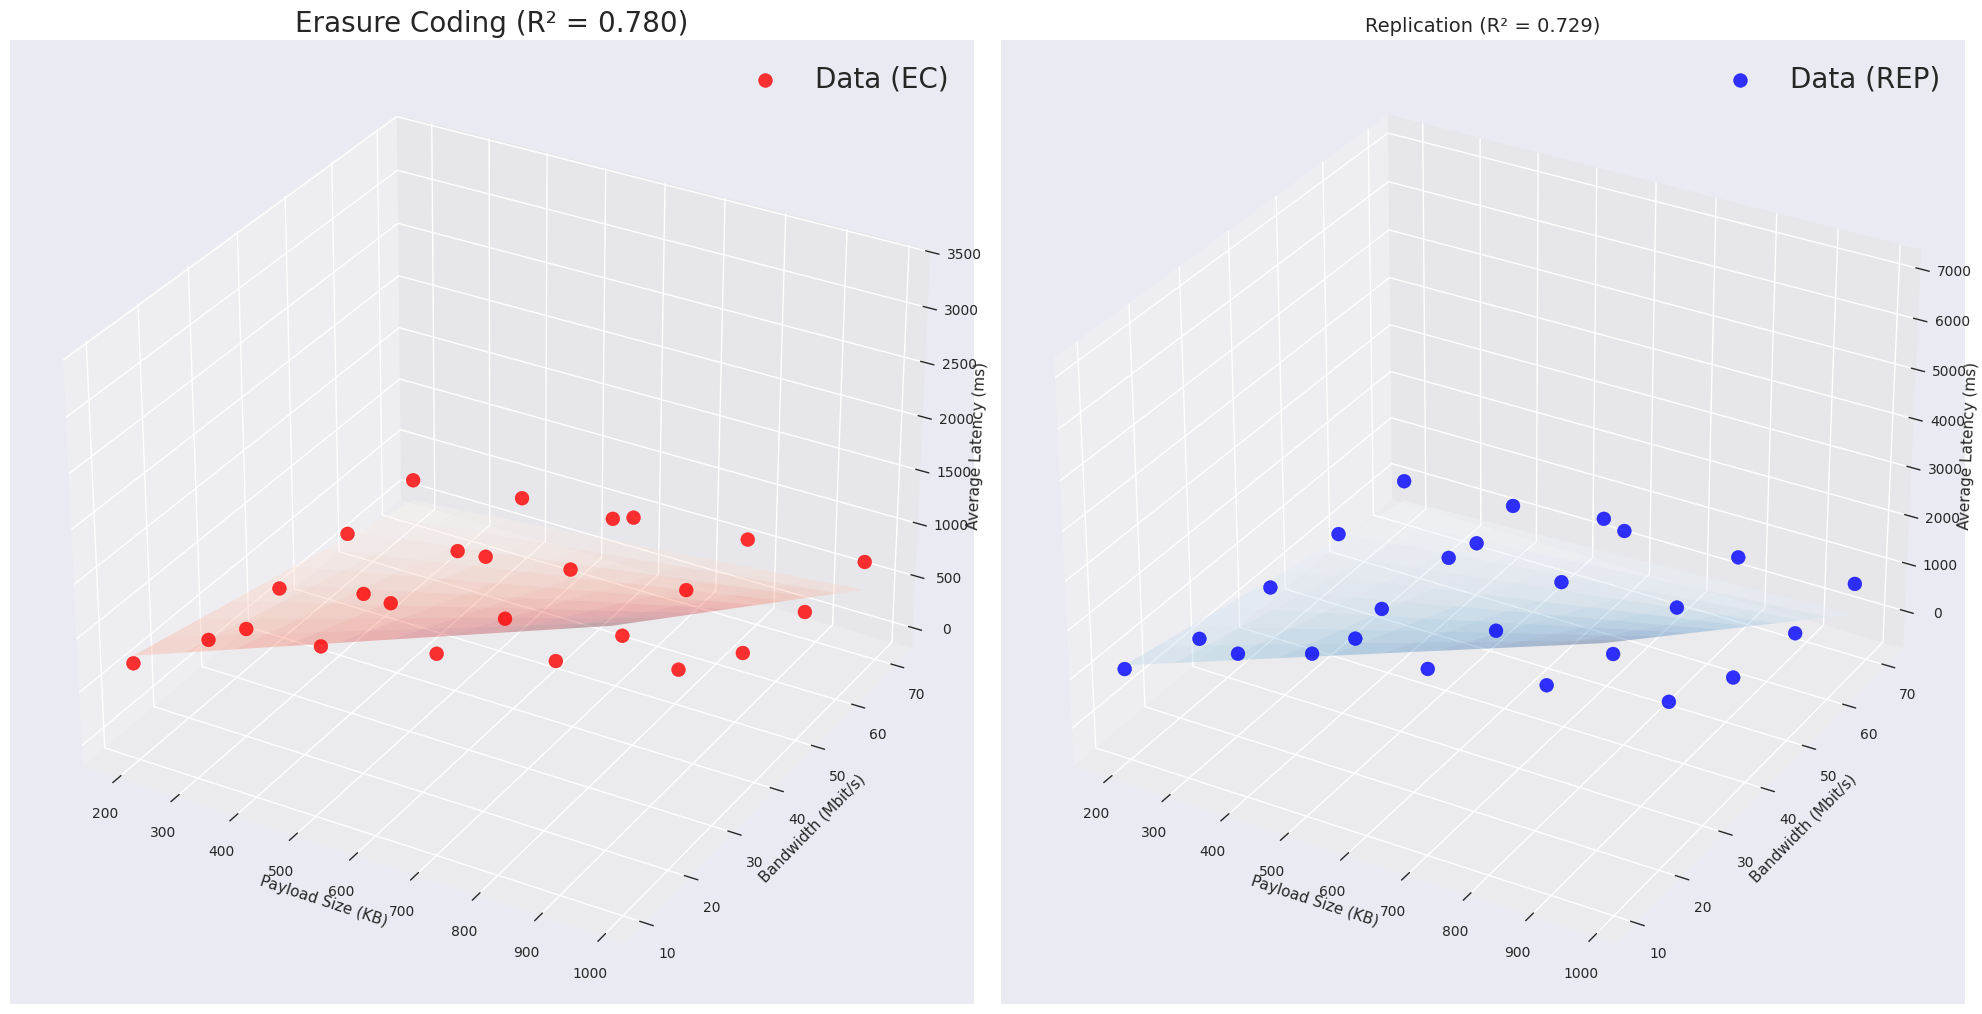
\includegraphics[width=\columnwidth]{resources/chapter-4/write_bigload_avgnet_regression.png}
\caption{Three-Dimensional Regression Model for Write Performance}
\label{fig:write-regression}
\end{figure}

The three-dimensional regression model shown in Figure \ref{fig:write-regression} employs ridge regression to handle the limited dataset and experimental noise. Separate models are constructed for erasure coding and replication response times as functions of bandwidth and payload size. The intersection of these surfaces defines the performance threshold boundary.

\begin{figure}[ht]
\centering
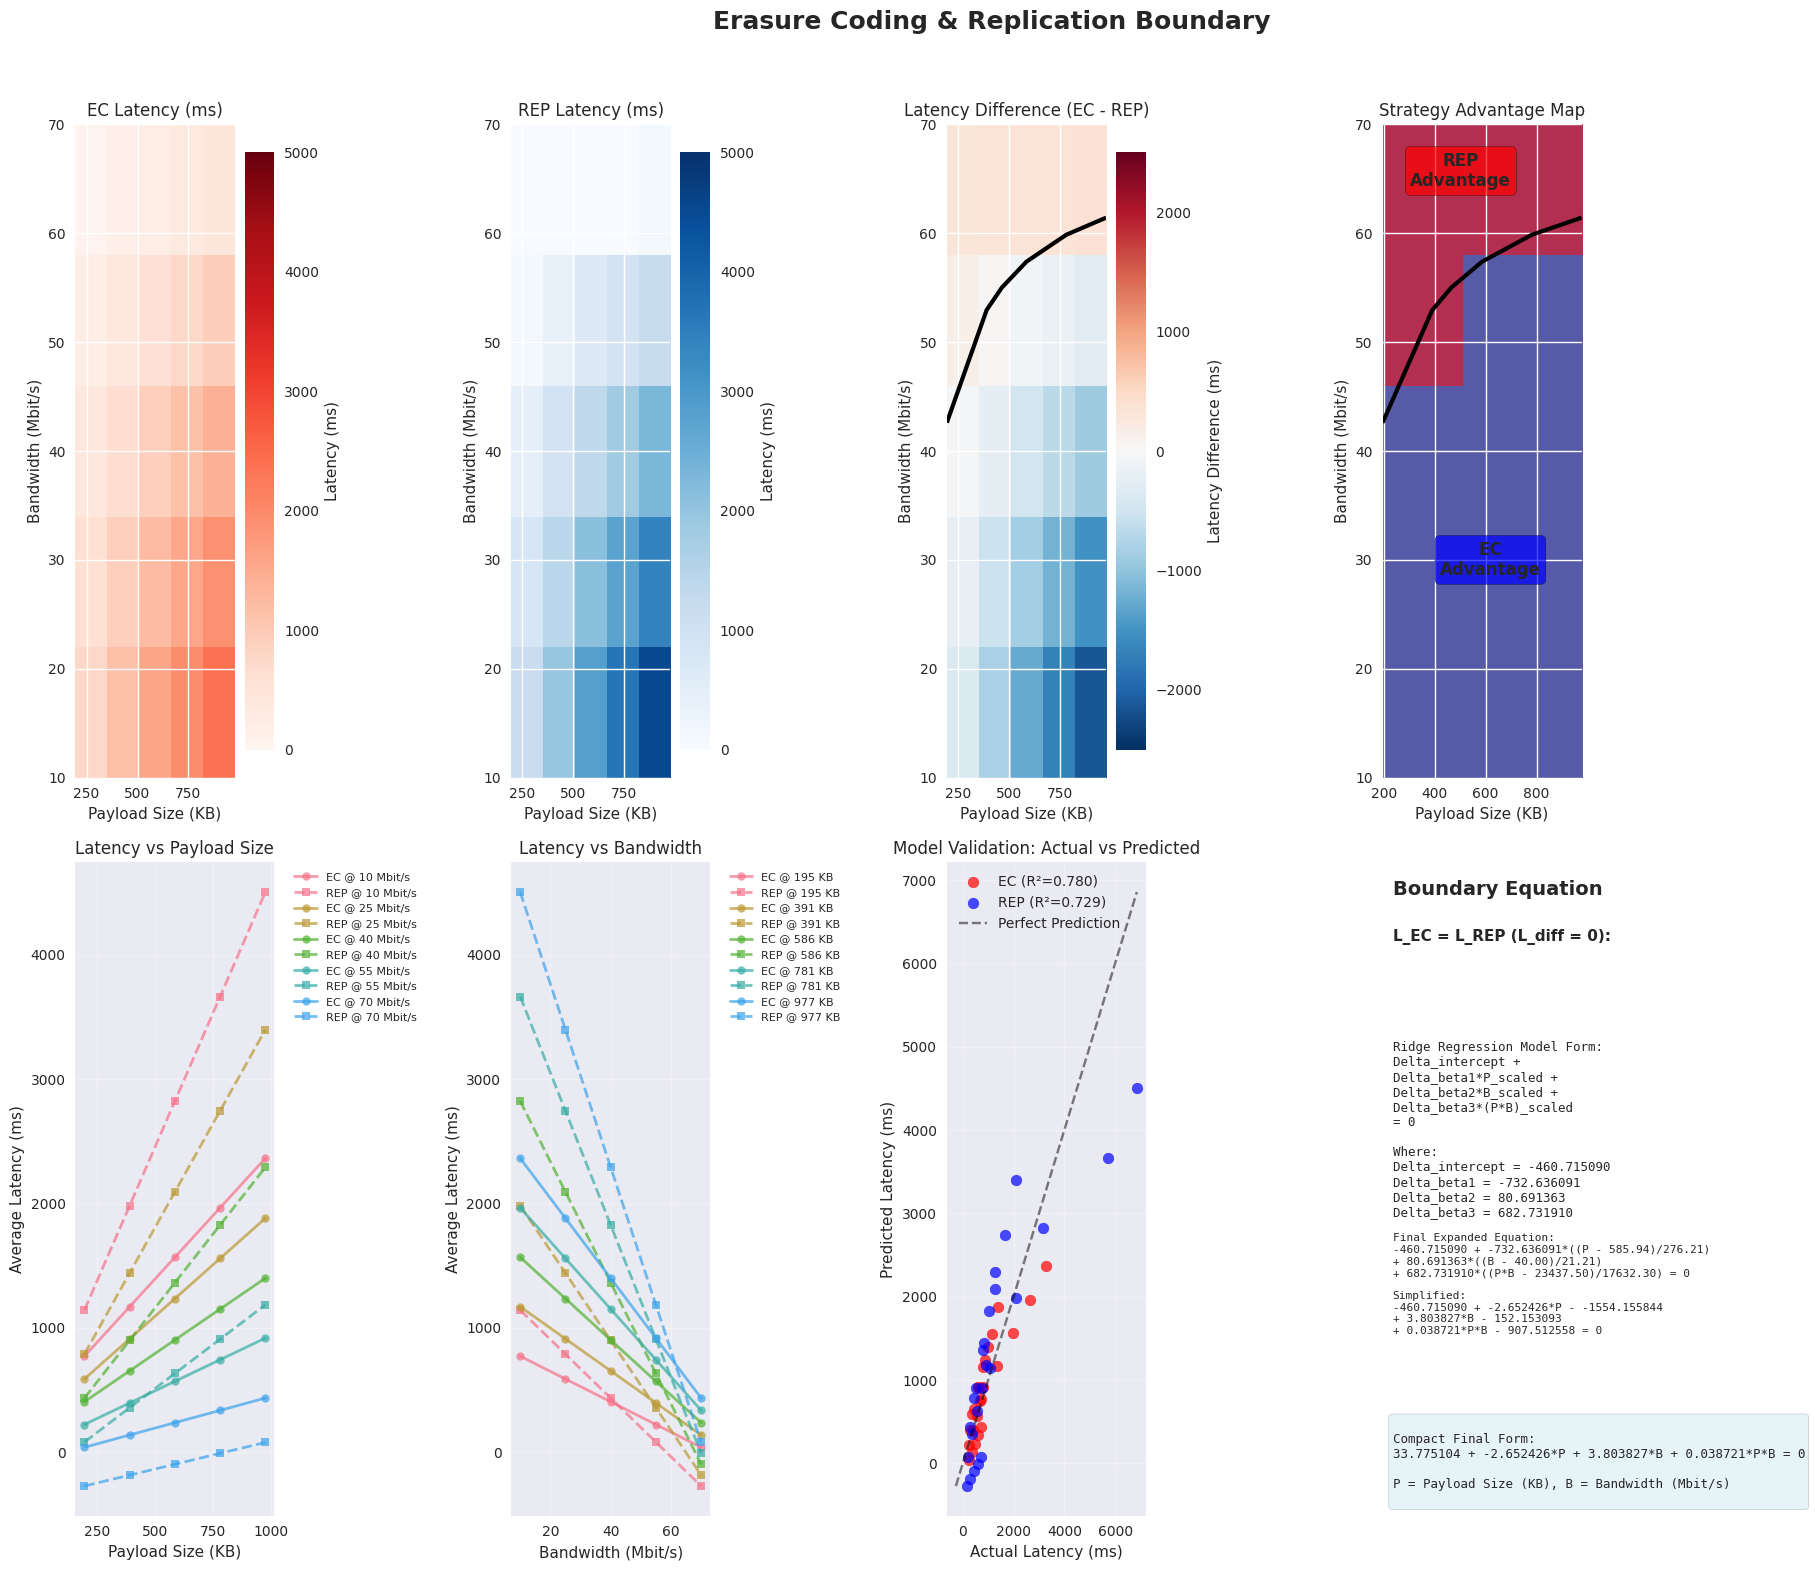
\includegraphics[width=\columnwidth]{resources/chapter-4/write_bigload_avgnet_boundary.png}
\caption{Performance Threshold Boundary Analysis}
\label{fig:write-boundary}
\end{figure}

The boundary curve analysis in Figure \ref{fig:write-boundary} derives a mathematical model for the performance crossover point. The curve represents conditions where erasure coding and replication achieve equivalent performance. Values above the curve favor erasure coding, while values below favor replication, enabling quantitative system selection decisions based on operational parameters.

\subsection{Read Operation Analysis}

Read operation analysis confirms the hypothesis that replication consistently outperforms erasure coding across all tested conditions. The mathematical foundation for this consistent advantage can be expressed as:

\begin{equation}
L_{EC} = T_{data} + T_{reconstruction} + T_{shard}
\end{equation}

\begin{equation}
L_{REP} = T_{data}
\end{equation}

\begin{equation}
\Delta L = T_{reconstruction} + T_{shard} > 0
\end{equation}

Where $\Delta L$ represents the additional latency inherent to erasure coding due to data reconstruction requirements. This overhead remains positive regardless of network conditions or payload size.

The implementation includes an in-memory store optimization that can reduce this penalty based on cache hit rates:

\begin{equation}
\Delta L = (T_{reconstruction} + T_{shard}) \times (1 - \text{hit rate})
\end{equation}

However, achieving 100\% hit rates is impractical due to memory constraints, maintaining replication's fundamental read advantage.

The read performance analysis across different scenarios confirms this consistent replication superiority. Figure \ref{fig:read-fastnet} demonstrates that even in high-bandwidth environments with small payloads, replication maintains lower response times than erasure coding due to the absence of reconstruction overhead.

\begin{figure}[ht]
\centering
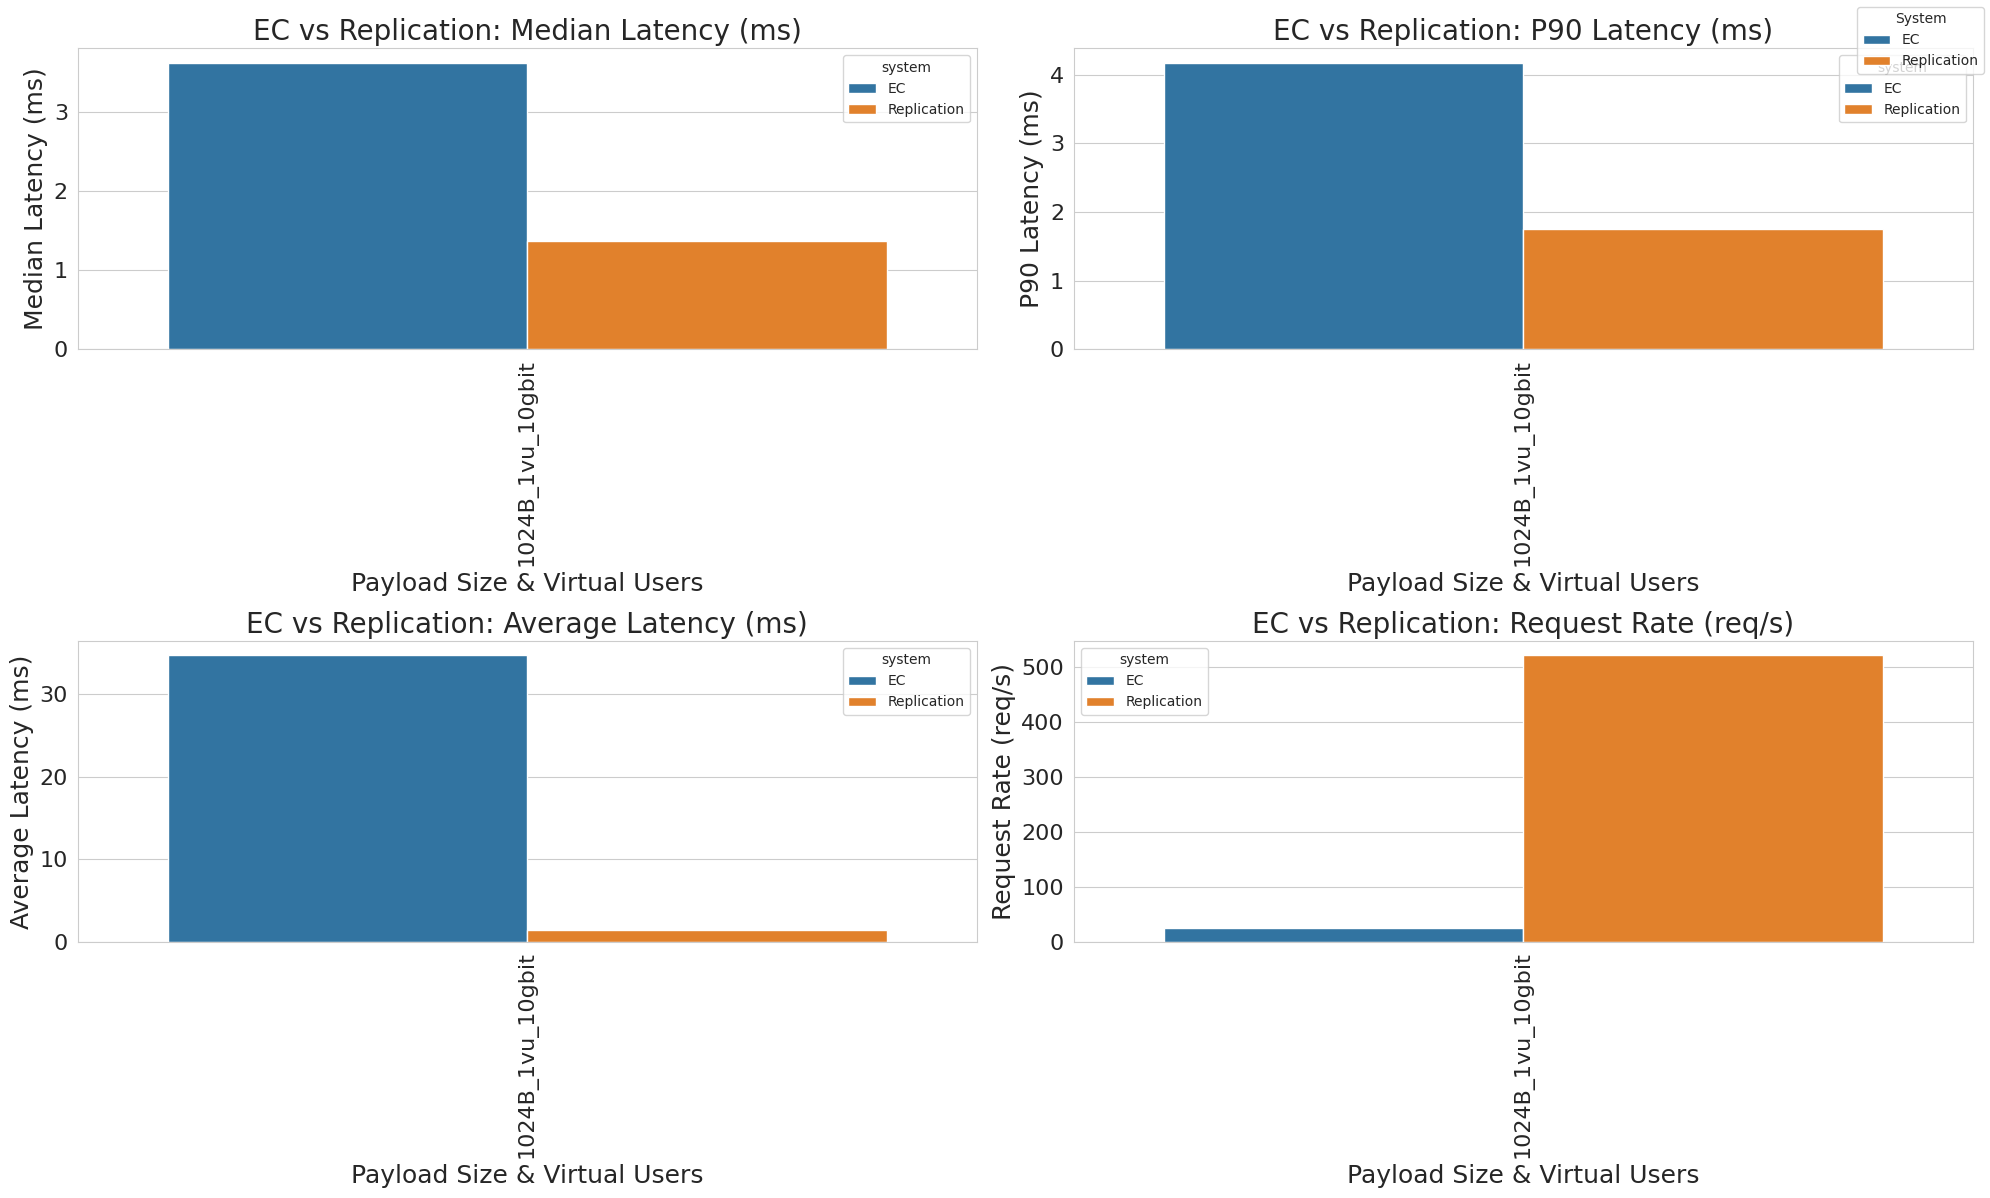
\includegraphics[width=\columnwidth]{resources/chapter-4/read_smload_fastnet.png}
\caption{Read Performance in High Bandwidth Environment}
\label{fig:read-fastnet}
\end{figure}

Similarly, Figure \ref{fig:read-slownet} shows that even under bandwidth-constrained conditions with large payloads—where erasure coding excels in write operations—replication continues to outperform erasure coding for read operations. This finding is particularly significant because it demonstrates that the conditions favoring erasure coding in write scenarios do not translate to read performance benefits. The reconstruction process required by erasure coding consistently adds latency regardless of network conditions, as the system must gather sufficient data shards from multiple nodes and perform computational reconstruction before delivering the result to the client. This overhead remains constant and unavoidable, creating a fundamental performance penalty that cannot be mitigated through network optimization or payload size adjustments.

\begin{figure}[ht]
\centering
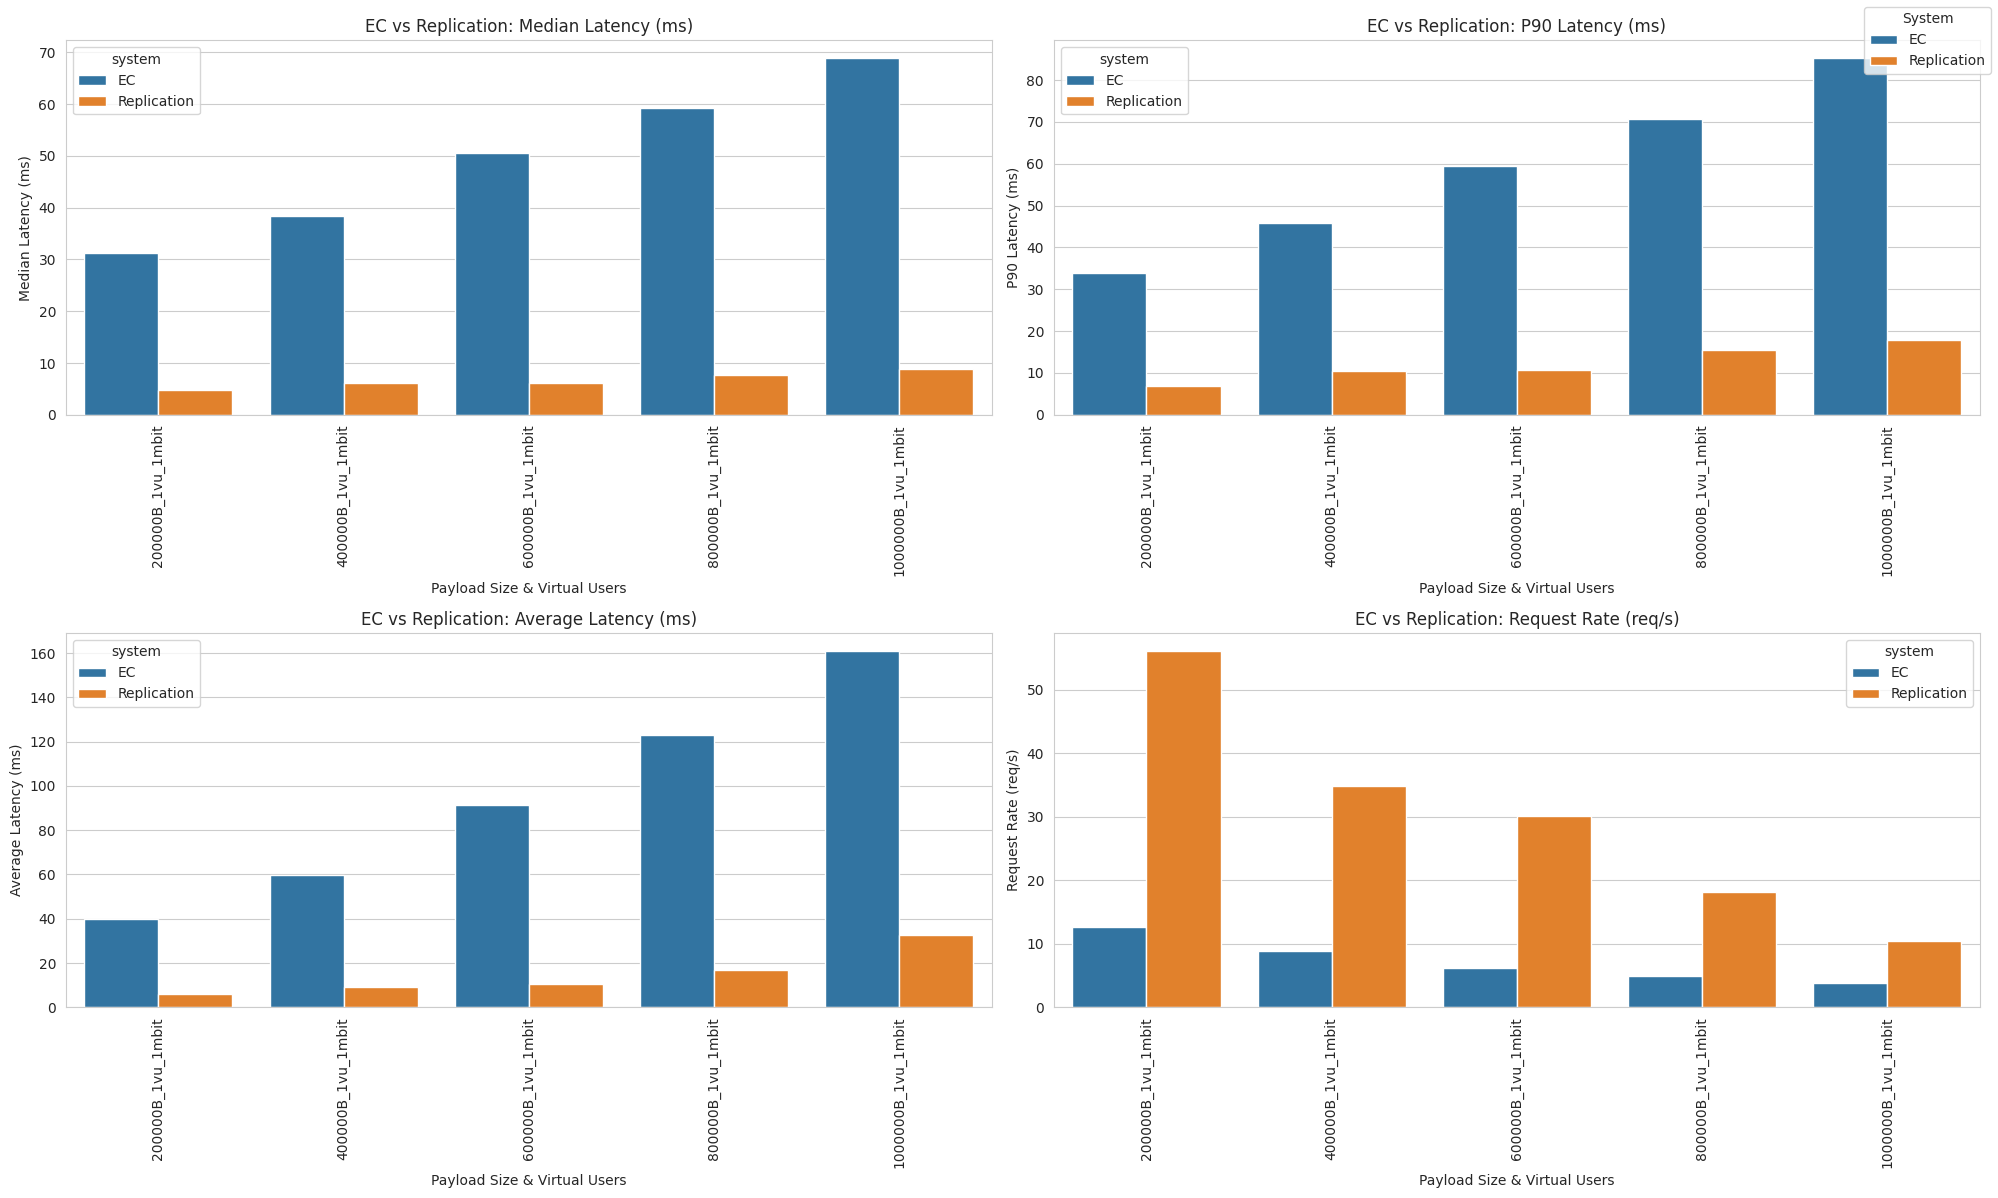
\includegraphics[width=\columnwidth]{resources/chapter-4/read_bigload_slownet.png}
\caption{Read Performance in Low Bandwidth Environment}
\label{fig:read-slownet}
\end{figure}

The comprehensive heatmap analysis in Figure \ref{fig:read-heatmap} visualizes this consistent pattern across all tested parameter combinations. Unlike the write operation heatmap which shows distinct regions favoring each approach, the read heatmap displays uniform replication superiority across the entire parameter space.

\begin{figure}[ht]
\centering
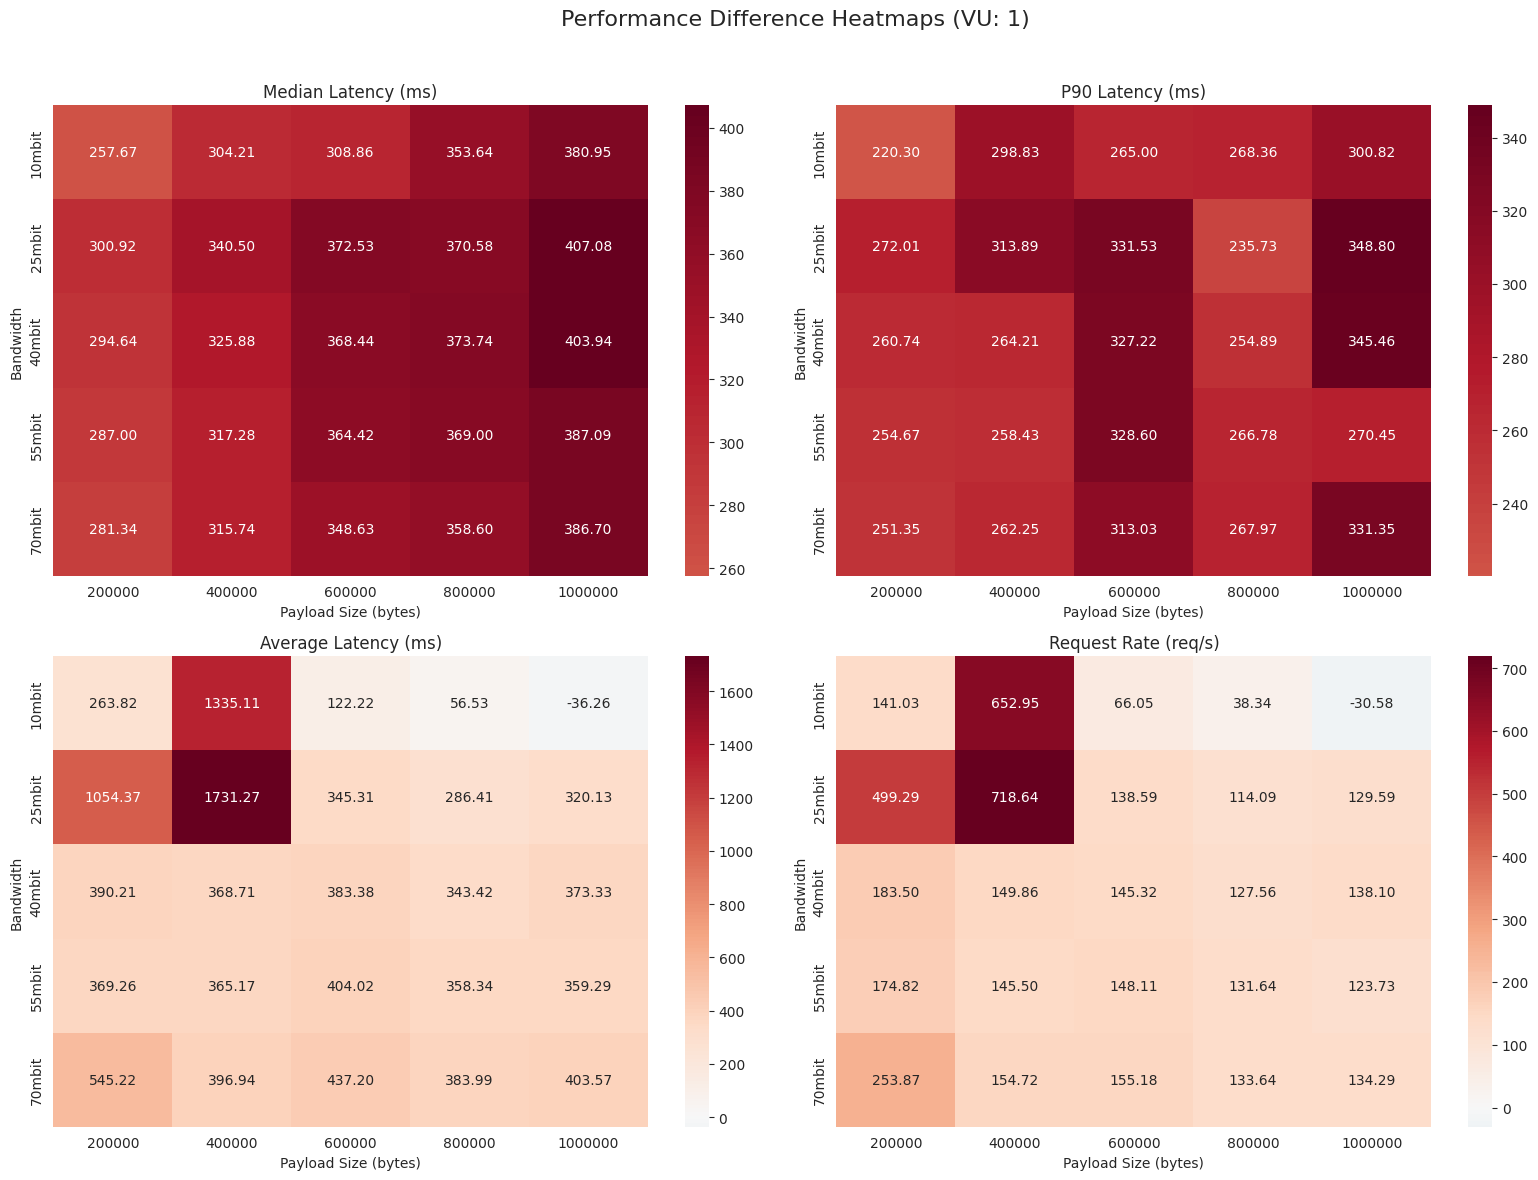
\includegraphics[width=\columnwidth]{resources/chapter-4/read_bigload_avgnet_heatmap.png}
\caption{Read Performance Heatmap Analysis}
\label{fig:read-heatmap}
\end{figure}

Figure \ref{fig:read-line} provides a line chart comparison that illustrates the performance gap between erasure coding and replication across different conditions. The visualization clearly shows the persistent performance advantage of replication, with response times consistently lower than erasure coding across all tested parameter combinations. The parallel trajectories of the performance curves indicate that no convergence point exists, mathematically confirming the absence of a performance threshold for read operations. This contrasts sharply with the write operation analysis where performance curves intersect at specific conditions. The consistent separation between the curves demonstrates that the fundamental overhead of data reconstruction in erasure coding systems cannot be overcome through parameter optimization, making replication the universally preferred choice for read-intensive workloads regardless of network or payload characteristics.

\begin{figure}[ht]
\centering
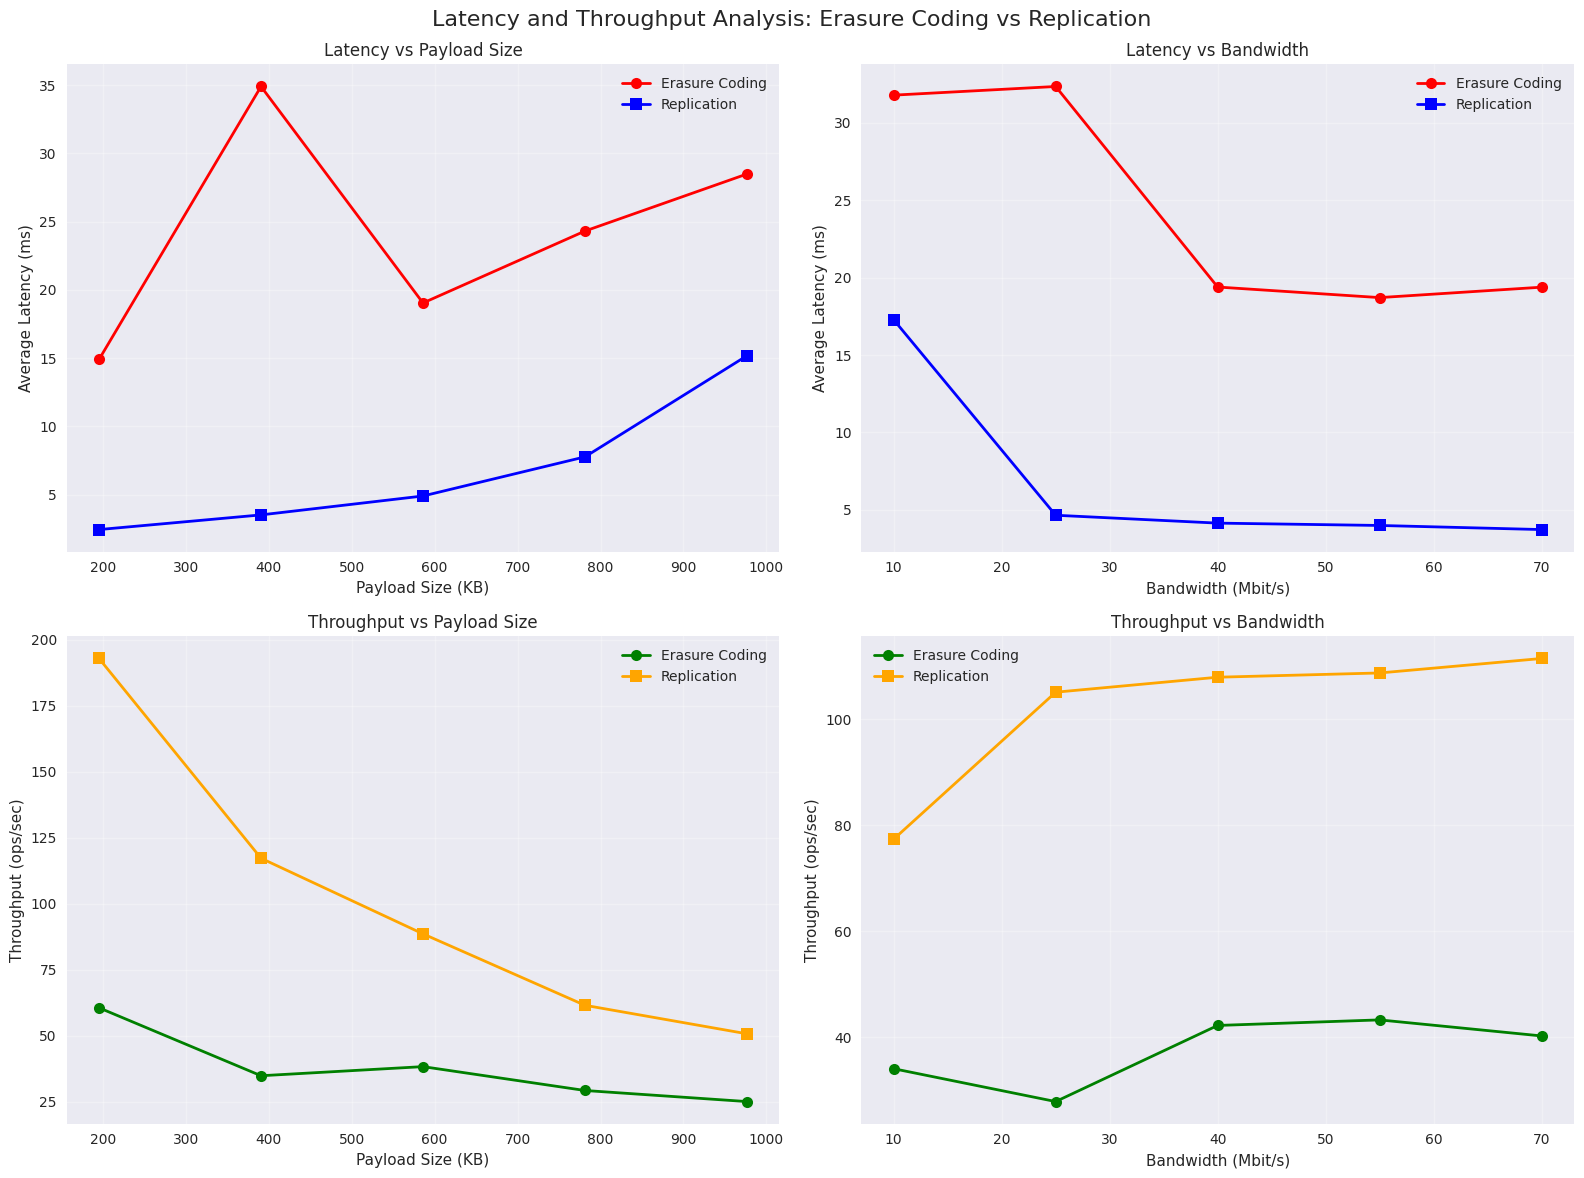
\includegraphics[width=\columnwidth]{resources/chapter-4/read_bigload_avgnet_line.png}
\caption{Read Performance Comparison Across Conditions}
\label{fig:read-line}
\end{figure}

\subsection{Performance Threshold Analysis}

The experimental results establish a clear performance threshold for write operations. Erasure coding demonstrates superior performance when:
- Payload size exceeds the threshold defined by the boundary curve
- Network bandwidth is sufficiently limited
- The ratio of encoding overhead to transfer time savings favors erasure coding

For read operations, no such threshold exists - replication maintains consistent superiority across all tested conditions due to the unavoidable reconstruction overhead in erasure coding systems.

\section{Discussion}

The experimental results provide comprehensive insights into the performance characteristics of erasure coding versus replication in distributed key-value store systems. The findings reveal a nuanced performance landscape that challenges simplistic assumptions about system optimization.

\subsection{Threshold Performance Validation}

The research successfully validates the existence of a performance threshold for write operations where erasure coding can outperform replication. This threshold is mathematically definable through the boundary curve derived from regression analysis, providing a practical tool for system architects to make informed decisions based on expected workload characteristics.

The threshold occurs when the computational overhead of erasure coding ($T_{encoding}$) is offset by the reduced network transfer time due to smaller data volumes. This relationship is environment-dependent and varies with hardware capabilities, network infrastructure, and data characteristics.

\subsection{Asymmetric Performance Characteristics}

A critical finding is the asymmetric nature of performance benefits between read and write operations. While write operations exhibit threshold behavior as demonstrated in Figures \ref{fig:write-heatmap} and \ref{fig:write-boundary}, read operations show consistent replication superiority across all conditions as evidenced in Figures \ref{fig:read-fastnet}, \ref{fig:read-slownet}, \ref{fig:read-heatmap}, and \ref{fig:read-line}. This asymmetry stems from the fundamental requirement for data reconstruction in erasure coding systems and has significant implications for system design:

\begin{itemize}
\item Systems with write-heavy workloads may benefit from erasure coding under appropriate conditions
\item Read-intensive applications consistently favor replication
\item Mixed workloads require careful analysis of read/write ratios and access patterns
\end{itemize}

\subsection{Practical Implementation Considerations}

The research reveals several practical considerations for real-world deployments:

\begin{itemize}
\item \textbf{Data Center Environments:} High-bandwidth, low-latency networks with predominantly small payloads favor replication. The computational overhead of erasure coding cannot be justified when network transfer times are minimal.
\item \textbf{Edge Computing and IoT:} Bandwidth-constrained environments with larger data objects can benefit from erasure coding's reduced network utilization, despite computational overhead.
\item \textbf{Hybrid Approaches:} The clear threshold boundary suggests potential for adaptive systems that dynamically select between erasure coding and replication based on current network conditions and data characteristics.
\end{itemize}

\subsection{Storage Efficiency Trade-offs}

While performance analysis focuses on response time, storage efficiency remains a crucial factor. Erasure coding provides significant storage savings compared to replication, which must be weighed against performance implications. For the tested configuration (4 data shards, 2 parity shards), erasure coding achieves approximately 33\% storage efficiency improvement over 3-way replication.

\subsection{Limitations and Model Validity}

The regression model and boundary curve are valid within the experimental conditions and may not generalize to different hardware configurations, network topologies, or erasure coding parameters. The model does not account for:

\begin{itemize}
\item CPU performance variations
\item Memory hierarchy effects
\item Disk I/O characteristics
\item Network topology complexity
\item Failure recovery scenarios
\end{itemize}

Future work should validate these findings across diverse hardware platforms and network configurations to establish broader applicability.

\subsection{Implications for Distributed Key-Value Stores}

For typical distributed key-value store applications characterized by small objects and high-performance data center networks, replication emerges as the preferred approach. Erasure coding becomes viable only in specialized scenarios with large objects or bandwidth constraints.

The research suggests that erasure coding adoption in key-value stores should be carefully evaluated against specific deployment characteristics rather than applied universally. The mathematical framework provided enables quantitative decision-making based on measured or expected system parameters.

\section{Conclusion}

This research provides a comprehensive performance analysis of erasure coding versus replication in distributed key-value store databases, establishing both theoretical foundations and practical guidelines for system design decisions. The analysis demonstrates that the choice between erasure coding and replication is not binary but depends on a complex interplay of system characteristics, workload patterns, and performance requirements.

\subsection{Key Results}

\begin{itemize}
\item \textbf{Write performance}: Erasure coding has an advantage for write operations when data objects are large and network bandwidth is low. In distributed key-value stores dominated by small objects, erasure coding is applicable only in the special case of sufficiently large objects and limited bandwidth; otherwise replication is preferable.
\item \textbf{Conditions for write improvement}: Based on the analysis, erasure-coded write response time is lower than replication when bandwidth and payload size for write operations are sufficiently large. No tested condition showed erasure coding outperforming replication for read operations.
\item \textbf{Storage efficiency}: For use cases with large objects, erasure coding reduces stored data volume compared to replication and thus reduces storage cost.
\end{itemize}

\subsection{Future Research Directions}

The research suggests several avenues for future investigation:

\begin{itemize}
\item \textbf{Recovery Analysis}: Erasure coding has a different recovery model compared to replication, which may impact performance and fault tolerance. Future work could explore the trade-offs involved in recovery strategies for both approaches.
\item \textbf{Additional Variables}: Future research could investigate other variables that impact the performance of erasure coding and replication, such as system configurations, hardware performance impacts, and system architecture.
\item \textbf{Hybrid Systems}: Development of systems that combines erasure coding and replication based on workload characteristics, network conditions, and performance requirements.
\item \textbf{Erasure Coding Optimizations}: The exploration of advanced erasure coding techniques, such as locally repairable codes and adaptive coding strategies, to enhance performance and reduce overhead.
\item \textbf{Real-world Validation}: Validation in actual production environments to verify the analysis result under real-world conditions with complex failure patterns and varying workloads.
\end{itemize}

The implementation and experimental artifacts are available in the project's open-source repository \cite{ajiw2025distkv}.